\section{System Description}

% describe overall system
As input, our system for retrieving follow-up questions requires: 1) an inadequate bug
report of interest; 2) a corpus of already posed follow-up questions extracted
from GitHub issues, including their corresponding bug reports and answers. As output, our system
produces a ranked list of follow-up questions appropriate to the inadequate bug report.
In this section, we describe our system, including how we create as a input
a large corpus of follow-up questions to recommend, how we select candidate follow-up questions from
this corpus for a specific incomplete bug report, and how we rank these questions in descending order of
their potential utility to the bug report.

\subsection{Selecting a Corpus of Bug Reports}


\begin{figure*}[ht]
\centering
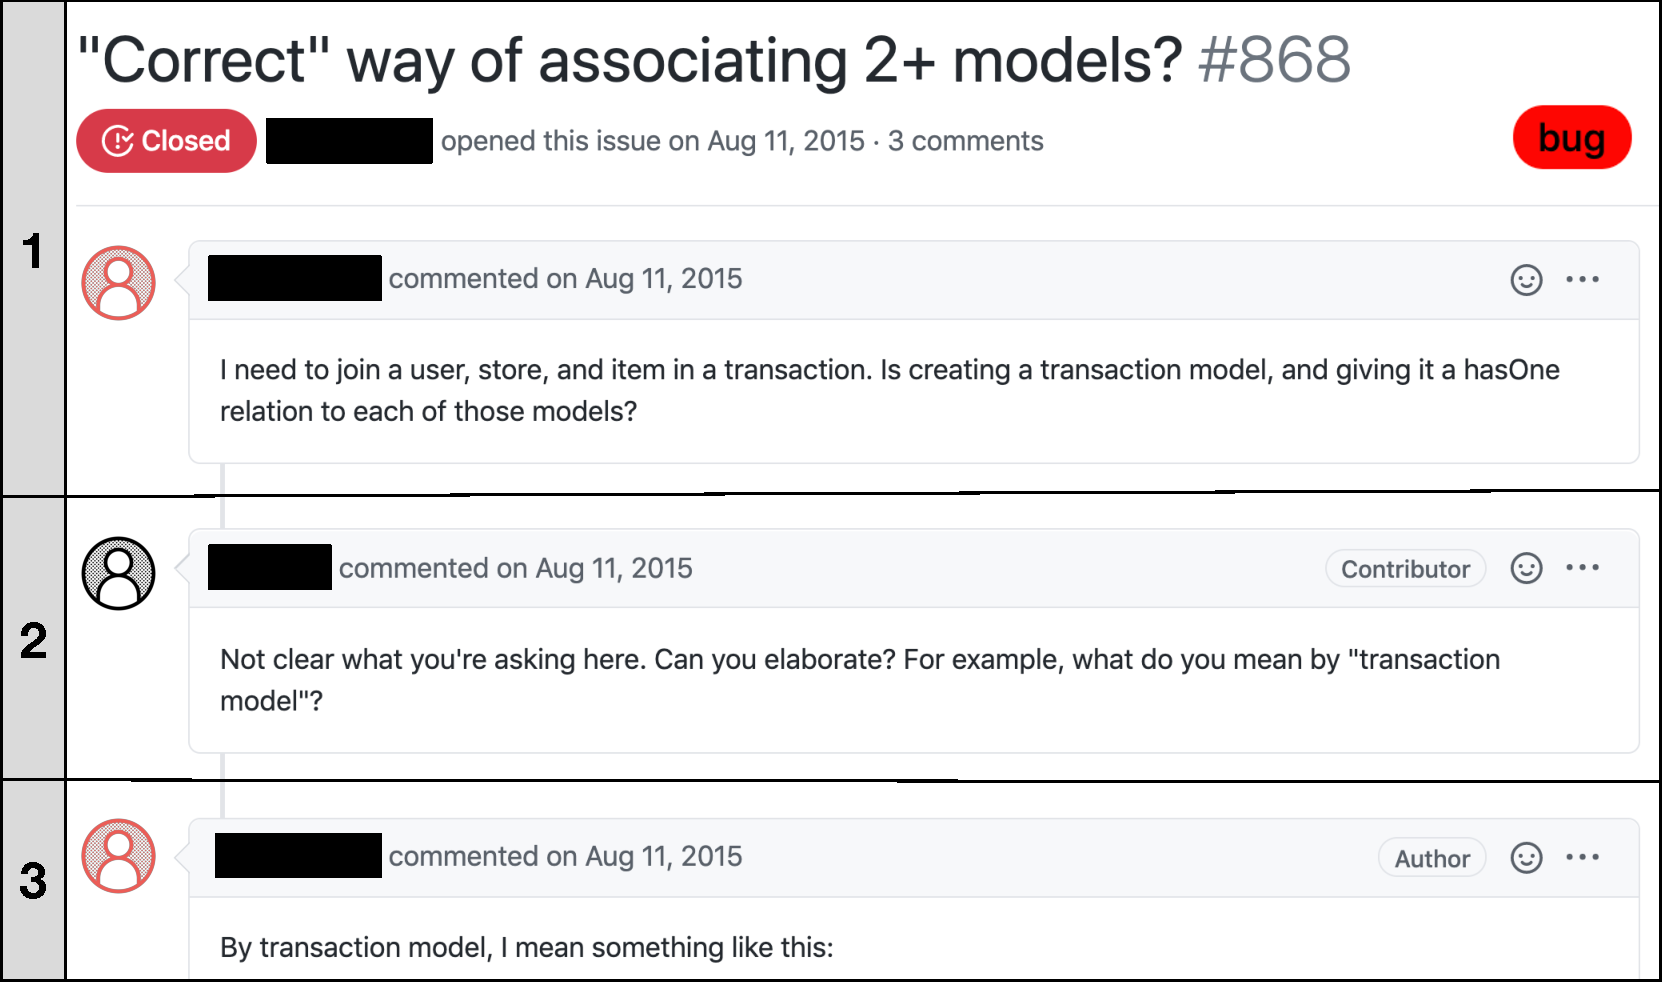
\includegraphics[width=0.70\linewidth]{figures/sample_issue.pdf}
\caption{.}
\label{fig:sample_br}
\end{figure*}

% overview of the entire process
Our goal in curating a corpus of bug report-related follow-up questions and their answers
is to find a large, representative and high-quality corpus. Manually curated corpora are of
high quality but they are difficult to scale-up. Automatic curation can easily scale but it
can be affected by significant noise, leading to low data quality, unless care is taken
to filter and sample follow-up questions in a way that noise is mitigated. As corpus size
is an important factor in our system, we opt for an automated approach with numerous filters
to ensure the data is of highest possible quality. With the number of active repositories available
on GitHub providing a very large input space, we can afford to be err on the side of being overly
restrictive in our filtering.

To automatically curate a corpus, we start by selecting GitHub repositories that have high bug reporting activity,
as measured by the number of issues created by non-contributors over some fixed period of time.
We select issues in those bug repositories that contain rapidly asked and succinct follow-up
questions, looking in the GitHub issue comments for these responses. Finally, because our system leverages
the answers of follow-up questions for ranking, we look for
a subsequent rapid answer to the follow-up question, encoded as either another comment or as an edit to the
original issue.

% list of more detailed steps to implement the plan
In more detail, we used the following set of steps and heuristics to curate the corpus:
\begin{enumerate}
\item We scraped a set of public GitHub repositories, sorted by the number of
non-contributor created issues, where a non-contributor is a GitHub user that has never
committed any code in the specific repository. In order to somewhat constrain the amount of repositories,
we focused on longer-running projects, specifically, created between 2008-2014, and recently
active with new issues created in the repository after Jan 1, 2019.
\item For each repository, in their sorted order from the previous step, we selected issues in the GitHub issue tracker
that are labeled as "bug", "crash", "fix" or unlabeled. We further selected only issues that contain follow-up questions as one of the issue comments (Step 2 in Figure~\ref{fig:sample_br}).  Follow-up questions were identified as sentences starting with a question word and ending with a question mark. In order to ensure we selected follow-up questions and not just
any questions, we constrained our selection based on time. That is, the comment containing the follow-up question must be posted
within 60 days of the issue creation date and must occur as a comment immediately following the post. As an additional safety mechanism,
we ensured that the comment was authored by a different user from the author of the issue. In selecting GitHub issues
we didn't use issue labels (or tags), e.g., to focus only on issues labeled as "bug", because we observed the labels were not
used consistently enough across most repositories.
\item The set of issues and candidate follow-up questions from the previous step were further filtered to
ensure an answer was provided. A key characteristic of the answer that we searched for is that it was authored
by the original issue creator. We allowed for answers to be posted as comments, as long as they occurred as the next sequential comment
to the follow-up question. We also allowed for answers to be encoded as edits to the original issue text, which we limited to add at least 4 additional words to avoid minor spelling or grammar modifications.
\end{enumerate}

Finally, we stopped the collection process when we gathered a dataset of 25KGitHub issues, which we deemed to be
sufficient for our purpose. Each data point is a triple of
issue, follow-up question, and answer. Together, the 25K triples form the primary corpus we use to
retrieve and rank follow-up questions for a given inadequate bug report.

\subsection{Selecting Candidate Follow-Up Questions for an Incomplete Bug Report}

Given the corpus of follow-up questions and an specific incomplete bug report of interest, selecting the
most likely candidate follow-up questions can be formed as an information retrieval
problem. That is, given the incomplete bug report as a query and an inverted index
created from the corpus (using Lucene), by using tf*idf as the ranking mechanism we
retrieve a set of 10 candidate follow-up questions, including also their original issue
and answer.

More specifically, we create a Lucene index by following this set of steps
on the corpus.
\begin{itemize}
\item {\em Filtering.} Removing code or stack traces from bug reports in our index allows
for more accurate matching. GitHub issues use markdown so we remove all text surrounded
by triple-quotes as this is typically how source code and stack traces are encoded. We also
remove quoted text (i.e., lines that start with the greater than symbol) as these typically
refer to some external information, which, again, is often stack traces, code, or project documentation.
\item {\em Tokenizing.} We perform standard tokenization used in software engineering applications
of information retrieval (cite). We tokenize on white space, remove punctuation (except for horizontal dashes)
and split on camel case and dashes, while also keeping the original unsplit tokens.
\item {\em Indexing.} We use Lucene's standard configuration to index the title and the body separately,
in order to ensure better quality matches. In order to provide more context, we extract the tags that the bug report
is labeled with (e.g., {\em fix-later, abc}) and the tags the GitHub repository is tagged with
(e.g., {\em java, linux}). The former provides specifics on the issue while the latter usually denotes
technologies the project uses or categories it belongs to.
\end{itemize}

To create a query out of the incomplete bug report, we tokenize the query use the equivalent process to
the one we performed on the bug reports in the corpus.


\subsection{Ranking the Candidate Follow-Up Questions}

To rank the set of candidate follow-up questions for a specific bug report we reformulate
the notion of the Expected Value of Perfect Information (EVPI), initially proposed as a
neurally computed quantity by Rao et al., towards bug reports and their inadequacy. EVPI estimates
the value to the incomplete bug report of the answer to the follow-up question. We express
the EVPI of a specific follow-up question $q_{i}$ from our candidate set, given an inadequate
bug report $br$, as the product of the probability of obtaining a specific answer $a_{i}$ and
the utility that answer would provide to $br$, i.e., the utility of $br$ augmented by $a_{i}$.

\medskip
$EVPI(q_{i}|br) = P(a_{i}|q_{i},br) * U(br+a)$
\medskip

In other words, this formulation scales the utility of an answer to a follow-up question by the
likelihood we are to receive this answer, given the follow-up question and the bug report.
To compute the utility of the augmented bug report, $U(br+a)$, we resort to the pattern based
identification of the constituent pieces of a bug report (rxpected Behavior,...) proposed by Chaparro et al.
We implement 5 of the most common pattern from the pattern catalogue, which rely on key words
and part-of-speech tagging to ensure high precision.



%
% p(a_i|q_i,p_i) is estimated via a 5-layer feed-forward NN.
%
% U(p+a) = softmax(d_OB+d_EB+dS2R), where dOB = OBa_i - OBp, and similarly dEB and dS2R
%
% OB_x is the number of OB sentences in document x, as defined by Chaparro et al.
